\chapter{Resoluções dos exercícios}
\renewcommand\thechapter{}
\renewcommand\thesection{\arabic{section}}

Este capítulo apresenta um direcionamento para a resolução dos exercícios. O pensamento, resolução ou descrição esperados são apresentados de forma resumida. É recomendável ao aluno apresentar respostas com o maior detalhamento possível, para praticar o entendimento completo de cada questão. Este aspecto é especialmente importante para as questões discursivas e aquelas solicitadas como parte de trabalhos e pesquisas da disciplina.

\section{Definição, histórico e paradigmas}

\begin{solution}
Definições:
\begin{enumerate}[a.]
	\item \textbf{Inteligência.} Algumas das definições encontradas no dicionário para inteligência são ``\textit{A capacidade de adquirir e aplicar conhecimento}'', ``\textit{A capacidade de pensamento e razão}'' e ``\textit{A capacidade de compreender e lucrar com a experiência}''. Todas essas são respostas razoáveis, mas se quisermos algo quantificável, usaríamos algo como ``\textit{A capacidade de aplicar conhecimento para melhorar o desempenho em um ambiente}''.
	
	\item \textbf{Inteligência artificial.} A inteligência artificial é definida como o estudo e construção de agentes inteligentes que façam um bom desempenho em um determinado ambiente, para uma determinada arquitetura de agente.
	
	\item \textbf{Racionalidade.} A racionalidade é definida como propriedade de um sistema que faz a ``coisa certa'' dado o que ele sabe.
\end{enumerate}
\end{solution}

\begin{solution}
Não. Os resultados dos testes de QI se correlacionam bem com certas outras medidas, como o sucesso na faculdade, capacidade de tomar boas decisões em situações complexas ou a capacidade de aprender novas habilidades e assuntos rapidamente. Porém, isso é válido apenas se os testes são aplicados a seres humanos. O teste de QI não mede tudo. Um programa que é especializado apenas para testes de QI (e se especializou apenas para a parte de analogia) provavelmente funcionaria mal em outras medidas de inteligência.

Considere a seguinte analogia: Se um humano executar os 100\,m em 10 segundos, podemos descrevê-lo como muito atlético e esperar desempenho competente em outras áreas, como caminhar, saltar, corrida com obstáculos, e talvez jogar bolas. Mas não descreveríamos um Boeing 747 como muito atlético porque pode percorrer 100\,m em 0,4 segundos, nem esperamos que ele seja bom em corrida com obstáculos e jogar bolas.
\end{solution}

\begin{solution}
\textbf{Leitores de código de barra de supermercados.} Embora a varredura de código de barras seja, em certo sentido, uma visão por computador, estes não são sistemas de IA. O problema de ler um código de barras é uma forma extremamente limitada e artificial de interpretação visual, e foi cuidadosamente projetada para ser o mais simples possível, dada a limitação de hardware.

\textbf{Menus de voz de telefones.} Em certa medida. Por exemplo, tais menus tendem a usar vocabulários e recursos muito limitados, como os dígitos ``Sim'' e ``Não''. Além disso, eles se limitam ao controle projetado, o que simplifica o problema. Por outro lado, os programas devem lidar com um espaço não controlado de todos os tipos de vozes e sotaques. Além disso, eles devem interpretar diferentes vocabulários, o que certamente os classifica como sistemas inteligentes.
	
\textbf{Mecanismos de busca na Web.} Determinar a relevância de uma página Web em uma consulta é um problema de processamento de linguagem natural. Os mecanismos de busca como o ``Ask.com'', que agrupam as páginas recuperadas em categorias, usam técnicas de agrupamento e aprendizagem de máquina. Do mesmo modo, outras funcionalidades fornecidas pelos motores de busca usam técnicas inteligentes. Por exemplo, o corretor ortográfico usa uma forma de mineração de dados com base na observação das correções dos usuários de seus próprios erros ortográficos. Por outro lado, o problema de indexar bilhões de páginas da Web de forma a permitir a recuperação em segundos é um problema no projeto do banco de dados, e não na inteligência artificial.
	
\textbf{Algoritmos de roteamento da Internet que respondem dinamicamente ao estado da rede.} Há algo a ser dito para vê-los como agentes inteligentes que trabalham no ciberespaço. A tarefa é sofisticada, a informação disponível é parcial, as técnicas são heurísticas (não garantidamente otimizadas) e o estado do mundo é dinâmico. Tudo isso é característico de atividades inteligentes. Por outro lado, a tarefa está muito longe daquelas normalmente realizadas na cognição humana.
\end{solution}

\begin{solution}
O prêmio Loebner 2017 está nas fases finais, mas sem vencedores até o momento. A edição de 2016 foi vencida por Mitsuku (programa) e Steve Worswick (autor). O diálogo entre os juízes e o robô pode ser visto em \url{http://www.aisb.org.uk/media/files/LoebnerPrize2016/Mitsuku.pdf}. Pelo diálogo, pode-se perceber que o processamento de linguagem natural é fundamental para estabelecer uma comunicação inteligente entre os juízes e a máquina. Além disso, as perguntas exigem habilidades como a aprendizagem de máquina, representação do conhecimento, raciocínio, etc. É possível conversar com este robô em \url{http://www.mitsuku.com/}. Mais detalhes sobre as edições do prêmio Loebner podem ser consultados em \url{http://www.aisb.org.uk/events/loebner-prize}.
\end{solution}

\begin{solution}
Observações:
\begin{enumerate} [a.]
	\item  \textbf{Tênis de mesa.} Um nível razoável de proficiência foi alcançado pelo robô de~\citet{Andersson1988}.
	
	\item \textbf{Dirigir no centro de Cairo.} Sim. Apesar dos desafios que os pesquisadores de veículos autônomos ainda precisam superar, todas as grandes dificuldades já foram vencidas e a tarefa de condução autônoma já é uma realidade. Em países como Estados Unidos e Alemanha os investimentos resultaram em vários veículos autônomos circulando pelas cidades.
	
	\item \textbf{Compras no mercado.} Não. Nenhum robô pode atualmente juntar as tarefas necessárias para esta atividade, como se deslocar em um ambiente lotado, usar a visão computacional para identificar uma grande variedade de objetos, coletar os objetos desejados sem danificá-los, etc. As tarefas individuais são possíveis, mas seria necessário um grande esforço de integração para juntar tudo.
	
	\item \textbf{Compras na Internet.} Sim. Robôs de software são capazes de lidar com tais tarefas, especialmente se a estrutura do site de compras na Web não muda radicalmente ao longo do tempo.
	
	\item \textbf{Jogar \textit{bridge}.} Sim. Programas como o GIB (veja detalhes em \url{http://www.gibware.com/}) jogam em um nível sólido.
	
	\item \textbf{Prova de teoremas.} Sim. Por exemplo, o cálculo da álgebra de Robbins.
	
	\item \textbf{Escrever uma história engraçada.} Não. Enquanto algumas prosas e poesias geradas por computadores são histericamente engraçadas, isso é invariavelmente não intencional, exceto no caso de programas que retornam a prosa que memorizaram.
	
	\item \textbf{Assessoria jurídica.} Sim, em alguns casos. A inteligência artificial tem uma longa história de pesquisa em aplicações de raciocínio jurídico automatizado. Dois exemplos notáveis são os sistemas especialistas baseados em Prolog utilizados no Reino Unido para orientar os membros do ministério público a lidar com as leis de seguridade social e nacionalidade. É previsto que o sistema de seguridade social do governo do Reino Unido tenha economizado aproximadamente U\$ 150 milhões em seu primeiro ano de operação. Contudo, a extensão a áreas mais complexas, como o direito dos contratos, prevê uma codificação satisfatória da vasta rede de conhecimentos de bom senso relativos a transações, práticas e acordos comerciais.
	
	\item \textbf{Tradução de idiomas.} Sim. De forma limitada, isso já está sendo feito e tem evoluído com o passar do tempo, sobretudo pelas técnicas de aprendizagem de máquina que melhoram o desempenho das traduções com base nos dados de experiências passadas.
	
	\item \textbf{Operação cirúrgica.} Sim. Os robôs são cada vez mais usados para a cirurgia, embora sempre sob o comando de um médico. As habilidades robóticas demonstradas em níveis sobre-humanos incluem perfuração de buracos no osso para inserir juntas artificiais, sutura e nó de amarração. Eles ainda não são capazes de planejar e executar uma operação complexa de forma autônoma do início ao fim.
\end{enumerate}
\end{solution}

\clearpage

\section{Agentes inteligentes}
\resetsolutionnumbering

\begin{solution}
Ambientes de tarefa:
\begin{table}[h]
	\centering
	\small
	\rowcolors{2}{white}{gray!25}
	\begin{tabular}{L{2cm} L{3cm} L{3cm} L{2.9cm} L{2.9cm}}
		\hline
		\rowcolor{black}
		\color{white}\textbf{Agente} & \color{white}\textbf{Medida de desempenho} & \color{white}\textbf{Ambiente} & \color{white}\textbf{Atuadores} & \color{white}\textbf{Sensores} \\
		\hline
		Jogar futebol & Número de gols, tempo de posse de bola, número de faltas & Campo, traves, áreas, bola, outros jogadores & Pernas e braços robóticos & Câmera, sonar \\
		Compra de livros na Internet & Preço, qualidade do livro, prazo de entrega & Sites de vendas, grupos de venda em redes sociais & Cartão de crédito & Algoritmo de leitura de conteúdo da Web \\
		Jogar uma partida de tênis & Pontuação, tempo de partida & Quadra, rede, raquete, bola, adversário & Pernas e braços robóticos & Câmera, sonar \\
		Praticar tênis na parede & Tempo sem deixar a bola cair & Limites no solo, parede, raquete, bola & Pernas e braços robóticos & Câmera \\
		Realizar um salto em altura & Altura do salto & Obstáculo, pista & Pernas robóticas & Câmera \\
		Licitações de um item em um leilão & Compra do item, valor pago & Site do leilão, ofertas, compradores & Função de lance & Leitor do site do leilão \\
		\hline
	\end{tabular}
\end{table}
\end{solution}

\begin{solution}
Classificação dos ambientes:
\begin{enumerate}[a.]
	\item \textbf{Jogo de palavras cruzadas:} completamente observável, determinístico, sequencial, estático, discreto e monoagente.
	\item \textbf{Xadrez com relógio:} completamente observável, determinístico, sequencial, semi-dinâmico, discreto e multiagente.
	\item \textbf{Pôquer:} parcialmente observável, estocástico, sequencial, estático, discreto e multiagente.
	\item \textbf{Gamão:} completamente observável, estocástico, sequencial, estático, discreto e multiagente.
	\item \textbf{Veículo autônomo:} parcialmente observável, estocástico, sequencial, dinâmico, contínuo e multiagente.
	\item \textbf{Diagnóstico médico:} parcialmente observável, estocástico, sequencial, dinâmico, contínuo e monoagente.
	\item \textbf{Análise de imagens:} completamente observável, determinístico, episódico, semi-dinâmico, contínuo e monoagente.
	\item \textbf{Robô de seleção de peças:} parcialmente observável, estocástico, episódico, dinâmico, contínuo e monoagente.
	\item \textbf{Controlador de refinaria:} parcialmente observável, estocástico, sequencial, dinâmico, contínuo e monoagente.
	\item \textbf{Instrutor interativo de inglês:} parcialmente observável, estocástico, sequencial, dinâmico, discreto e multiagente.
\end{enumerate}
\end{solution}

\begin{solution}
Exercício de implementação.
\end{solution}

\begin{solution}
Exercício de implementação.
\end{solution}

\begin{solution}
Aspirador de pó com penalidade:
\begin{enumerate}[a.]
	\item Não. Se o agente possui percepção apenas do quadrado onde se encontra, ele não pode decidir sobre não mais se movimentar. Somente com a observação completa do cenário o agente reativo consegue verificar que todos os quadrados já estão limpos e, com isso, não mais se movimentar. Para ser racional com observação parcial, o agente deve manter em memória as percepções anteriores, deixando de ser um agente reativo simples.
	
	\item Sim. Conforme discutido no item anterior, se o agente pode manter em memória os demais quadrados do ambiente, ele passa a ser racional.
	\begin{itemize}
		\item \textbf{Medida de desempenho:} agente recebe 100 pontos para cada quadrado limpo ao fim do dia e -1 ponto para cada movimento.
		\item \textbf{Conhecimento do agente sobre o ambiente:} o agente conhece a geografia do ambiente e desconhece a distribuição da sujeira e sua posição inicial. Quadrados limpos permanecem limpos até o fim do dia. A ação de aspiração limpa o quadrado onde o agente se encontra. As ações \textit{esquerda} e \textit{direita} movem o agente para os quadrados adjacentes (conforme o lado escolhido). O agente não pode se movimentar para fora do ambiente. O agente mantém uma memória interna (modelo) com as percepções e ações anteriores.
		\item \textbf{Ações:} \textit{esquerda}, \textit{direita}, \textit{aspirar} e \textit{nada}.
		\item \textbf{Percepções:} agente percebe sua posição e se a posição contém sujeira.
		\item \textbf{Observações:} para a racionalidade, os fatos dos quadrados permanecerem limpos e da ação \textit{aspirar} ser perfeita são fundamentais.
	\end{itemize}
	
	\item Neste caso, um agente reativo simples pode ser perfeitamente racional. Cada percepção mostra o estado (limpo/sujo) de cada quadrado. Com isso, o agente pode agir, limpando um quadrado, por exemplo. A percepção seguinte apontará para o estado completo atualizado, tornando o agente racional.
\end{enumerate}
\end{solution}

\begin{solution}
Aspirador de pó aleatório:
\begin{enumerate}[a.]
	\item Não. Se o agente não conhece a geografia do ambiente, percebe apenas a sua localização e a sujeira deste local e ainda não armazena em memória o que acabou de fazer, ele não tem como tomar a decisão que maximiza sua função de desempenho. Por exemplo, ele ficará preso para sempre contra um parede quando tentar se mover e a direção estiver bloqueada. Para superar esta dificuldade, o agente deveria aplicar alguma aleatoriedade, mas isso não leva à racionalidade.
	
	\item Uma possibilidade é um agente que limpa a sujeira do quadrado onde se encontra e se move aleatoriamente. Esta abordagem supera um agente reativo simples, pois este último pode ficar preso infinitamente em uma ação, conforme discutido no item anterior. Logo, a aleatoriedade ajudaria a superar estas dificuldades. Isso é muito parecido com o que um aspirador \textit{Roomba} faz (apesar de que o \textit{Roomba} usa um sensor de toque e age aleatoriamente somente quando acerta um obstáculo). Ele funciona razoavelmente bem em ambientes compactos. Em ambientes que se assemelham a labirintos ou aqueles com passagens estreitas ele pode demorar bastante para cobrir todos os quadrados.
	\begin{itemize}
		\item Exercício de implementação.
	\end{itemize}
	
	\item O ambiente da figura abaixo apresenta dificuldade para um agente com aleatoriedade de movimento. A aleatoriedade dificulta superar os corredores para acesse de um quadrado a outro.
	
	\begin{figure}[h]
		\centering
		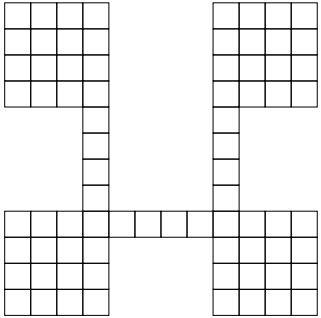
\includegraphics[width=0.5\textwidth]{img/exercicios/ambiente-dificil-aleatoriedade}
	\end{figure}
	
	\item Um agente reativo com estado pode construir internamente uma representação (mapa) do ambiente. Uma busca em profundidade encontrará todos os estados em tempo linear de acordo com o tamanho do ambiente. Portanto o agente pode ter um desempenho muito superior a um agente reativo.
	\begin{itemize}
		\item Exercício de implementação.
	\end{itemize}
\end{enumerate}
\end{solution}

\clearpage

\section{Buscas em espaços de estados}

\resetsolutionnumbering

\begin{solution}
Definições:
\begin{itemize}
	\item Um \textbf{estado} é a situação em que um agente pode se encontrar. Distinguimos dois tipos de estados: \textit{estado do mundo} -- as situações concretas no mundo real e \textit{estados de representação} -- representações abstratas do mundo real que são usadas pelos agentes nas decisões do que fazer.
	
	\item Um \textbf{espaço de estado} é um grafo cujos formam o conjunto de todos os estados possíveis e os arcos são ações que transformam um estado em outro (ou que levam o agente de um estado a outro).
	
	\item A \textbf{árvore de busca} é uma árvore (um grafo direcionado acíclico) na qual o nó raiz é o estado inicial e o conjunto de filhos de cada nó consiste nos estados alcançáveis na tomada de qualquer ação.
	
	\item Um \textbf{nó de busca} é um nó na árvore de busca.
	
	\item Uma \textbf{ação} é alguma coisa que o agente pode escolher fazer.
	
	\item O \textbf{objetivo} consiste no estado que o agente está tentando alcançar.
	
	\item O \textbf{modelo de transição}, também chamado de \textbf{função sucessor}, é especificado por uma função $sucessor(a, s)$ que devolve o estado que resulta de executar uma ação $a$ em um estado $s$.
	
	\item O \textbf{fator de ramificação} em uma árvore de busca é o maior número de sucessores que um nó pode conter.
\end{itemize}
\end{solution}

\begin{solution}
Um \textbf{estado do mundo} consiste em como a realidade é ou poderia ser. O estado do mundo pode ser \textit{Arad} ou \textit{Bucharest}, por exemplo. O estado do mundo inclui todo e qualquer detalhe do mundo real, como a rua em que estamos, o que está tocando no rádio e o preço do chá na China. Uma \textbf{descrição do estado} é a definição interna que um agente possui de um estado do mundo. Por exemplo, o agente precisa saber somente sua localização (\textit{Arad} ou \textit{Bucharest}), e não todos os detalhes que não influenciam na execução da tarefa desejada. Ou seja, essas descrições são aproximadas, mantendo apenas alguns aspectos do estado do mundo.  Precisamos diferenciar \textbf{estados do mundo} de \textbf{descrição do estado}, pois descrições de estados são abstrações do estado do mundo e podem conter perdas.

Os \textbf{nós de busca} são gerados durante a busca, representando um estado em que o processo de busca sabe como chegar. Eles contêm informações adicionais além da descrição do estado, como a sequência de ações usadas para alcançar esse estado. Essa distinção é útil porque podemos gerar diferentes nós de busca que possuem o mesmo estado, além de apresentarem mais informações que uma representação do estado.
\end{solution}

\begin{solution}
Problema de roteamento entre dois amigos.
	\begin{enumerate}[a.]
		\item Formulação:
		\begin{itemize}
			\item \textbf{Espaço de estados:} todos os pares possíveis de cidades $(i, j)$. O mapa não é o espaço de estados.
			
			\item \textbf{Função sucessor:} os sucessores de $(i, j)$ são todos os pares $(x, y)$, tal que $x$ seja adjacente de $i$ e $y$ seja adjacente de $j$.
			
			\item \textbf{Objetivo:} estar em $(i, i)$ para qualquer cidade $i$.
			
			\item \textbf{Custo de passo:} o custo de ir de $(i, j)$ para $(x, y)$ é $max(d(i, x), d(j, y))$.
		\end{itemize}
	
		\item No melhor caso, os amigos se dirigem um em direção ao outro em passos de tamanho igual. Isso reduz a separação entre eles por duas vezes o custo de cada passo. Portanto, as heurísticas (i) e (ii) superestimam o custo até a solução. A heurística (iii) é a única admissível.
	
		\item Sim. Um exemplo consiste em um mapa com dois nós conectados por um link. Os dois amigos trocarão de lugares para sempre. O mesmo vai acontecer em qualquer sequência se eles começarem em um número ímpar de passos separados.
	
		\item Sim. Dado um mapa sem solução da questão (c), podemos adicionar um auto-loop (caminho de um estado para si mesmo) a qualquer um dos nós. Se os amigos começam em um número ímpar de passos separados, um movimento no qual um dos amigos toma o auto-loop altera a distância em 1, tornando o problema solucionável. Se o auto-loop não for tomado, o argumento de (c) se aplica e nenhuma solução é possível.
	\end{enumerate}
\end{solution}

\begin{solution}
Formulação de problemas:
\begin{enumerate}[a.]
	\item Coloração de mapa
	\begin{itemize}
		\item \textbf{Estado inicial:} sem região colorida.
		\item \textbf{Teste de objetivo:} todas as regiões coloridas sem que duas regiões adjacentes contenham a mesma cor.
		\item \textbf{Função sucessor:} atribuir uma cor para uma região.
		\item \textbf{Função de custo:} número de atribuições.
	\end{itemize}
	
	\item Macaco e as bananas:
	\begin{itemize}
		\item \textbf{Estado inicial:} como descrito no enunciado.
		\item \textbf{Teste de objetivo:} macaco apanha as bananas.
		\item \textbf{Função sucessor:} subir no engradado; descer do engradado; mover engradado de um ponto a outro; caminhar de um ponto a outro; apanhar as bananas (apenas se puder alcançá-las).
		\item \textbf{Função de custo:} número de ações.
	\end{itemize}	
	
	\item Problema dos jarros:
	\begin{itemize}
		\item \textbf{Estado inicial:} jarras com valores $[0, 0, 0]$.
		\item \textbf{Função sucessor:} dados os valores $[x, y, z]$, gera $[12, y, z]$, $[x, 8, z]$, $[x, y, 3]$ (ação de enher); $[0, y, z]$, $[x, 0, z]$, $[x, y, 0]$ (ação de esvaziar); ou para quaisquer duas jarras com valores atuais $x$ e $y$, despeje $y$ em $x$; Isso muda a jarra com $x$ para o mínimo de $x + y$ e a capacidade da jarra, e diminui a jarra com $y$ pelo valor obtido pela primeira jarra.
		\item \textbf{Função de custo:} número de ações.
	\end{itemize}
	
\end{enumerate}
\end{solution}

\begin{solution}
Custos negativos nos caminhos:
\begin{enumerate}[a.]
	\item Qualquer caminho, por pior que pareça, pode levar a uma recompensa arbitrariamente grande (custo negativo). Portanto, seria necessário explorar todos os caminhos possíveis para se ter certeza que encontraria o melhor.
	
	\item Suponha que a maior recompensa possível é $c$. Então, se conhecemos a profundidade máxima do espaço de estados, qualquer caminho com $d$ níveis restantes pode ser melhorado por no máximo de $c \times d$. Sendo $x$ o custo do melhor caminho e $y$ o custo de um candidato, sabemos que o candidato poderá ter custo não inferior a $y + c \times d$. Logo, se $y + c \times d > x$, o caminho candidato pode ser podado. Para espaços de estados com loops esta garantia não ajuda, pois é possível dar uma volta a um loop várias vezes, escolhendo a recompensa $c$ a cada vez. 
	
	\item O agente deve planejar dar uma volta a esse ciclo para sempre (a menos que possa encontrar outro loop com uma recompensa ainda melhor).
	
	\item O valor associado a uma bela paisagem é menor quando ela é revisitada. Uma paisagem nunca vista provoca uma grande recompensa, mas o mesmo não acontece quanto ela é revisitada muitas vezes. Neste caso, a paisagem passa a ser entediante, não provocando nenhuma recompensa. Para implementar isso, devemos expandir o espaço de estados incluindo um estado com memória. A representação de um estado não inclui apenas a localização, mas um conjunto de localizações já visitadas. A recompensa por visitar uma nova localização é agora implementada por uma função do número de vezes que ela foi visitada anteriormente.
\end{enumerate}
\end{solution}

\begin{solution}
Missionários e canibais:
\begin{enumerate}[a.]
	\item Aqui está uma representação possível: um estado é uma tupla de 6 números inteiros, que correspondem à quantidade de missionários, canibais e barcos em cada lado do rio. O objetivo é um estado com 3 missionários e 3 canibais no segundo lado do rio. A função de custo é 1 para cada ação executada. Os sucessores de um estado são todos os estados, que configuram a movimentação de uma ou duas pessoas e um barco para o outro lado do rio.
	
	\item Exercício de implementação. O espaço de busca é pequeno, então qualquer algoritmo ótimo funciona. Isso é suficiente para eliminar movimentos que voltam para um estado já visitado.
	
	\item Não é evidente que quase todos os movimentos são inválidos ou revertem para um estado anterior. Existe uma sensação de um grande fator de ramificação e nenhuma maneira clara de prosseguir.
\end{enumerate}

\begin{figure}[h]
	\centering
	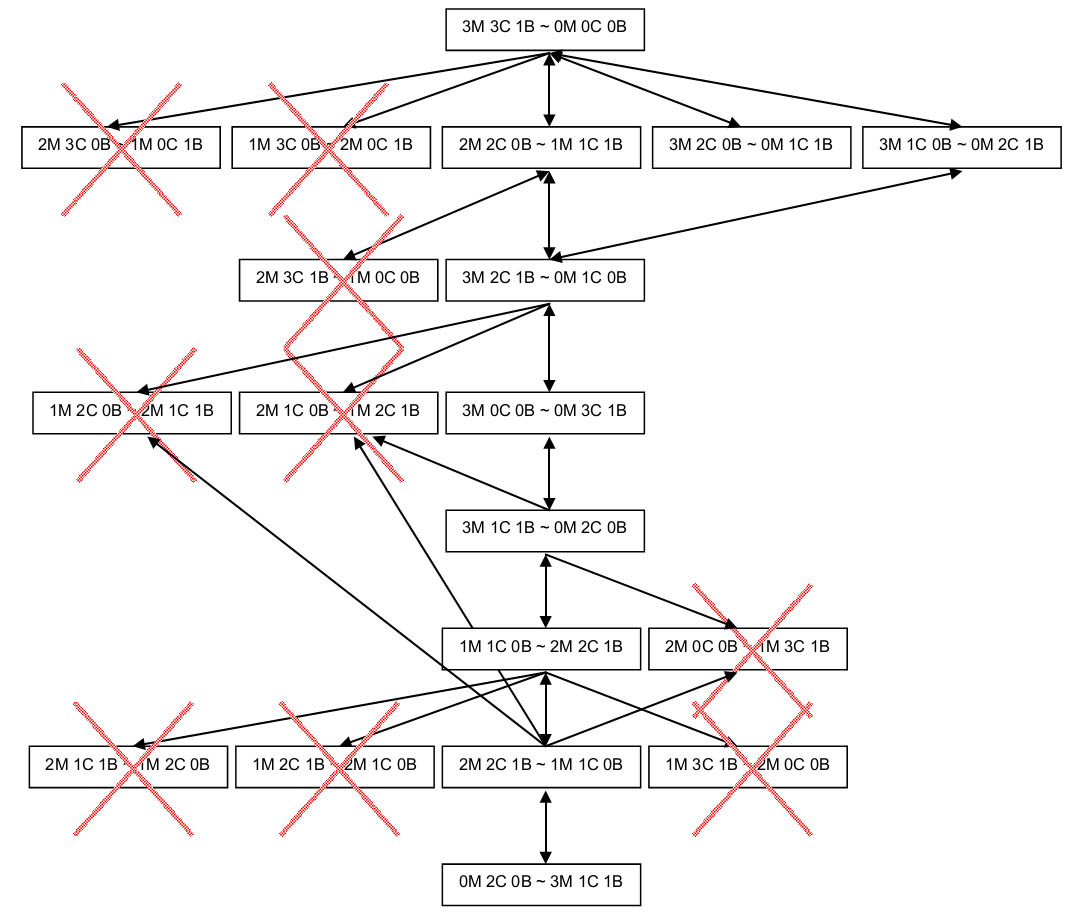
\includegraphics[width=0.85\textwidth]{img/exercicios/missionarios-canibais}
\end{figure}
\end{solution}

\insertspace
\insertspace

\begin{solution}
O espaço de estados é uma árvore com profundidade igual a 1, com todos os estados sendo sucessores do estado inicial. Não há distinção entre uma busca em largura e uma busca em profundidade nesta árvore. Se o comprimento da sequência for ilimitado, o nó da raiz terá infinitos sucessores, então um simples algoritmo de teste dos nós sucessores pode funcionar.

O que acontece depois depende de como as ações compostas são classificadas. Se não existe uma ordenação específica, então ocorre uma busca aleatória (porém sistemática) de possíveis soluções. Se eles são ordenados por ordem alfabética, é implementada uma busca em largura.

Uma importante desvantagem de suprimir o espaço de busca dessa forma, ocorre se descobrimos que um plano que inicia com a ação $x$ não compõe a solução. Neste caso, não existe uma maneira simpes de ignorar todas as outras ações compostas que iniciam com a ação $x$. Isto é um problema em particular para algoritmos de busca informados.

Descartar a estrutura de sequência não é uma abordagem particularmente prática para a pesquisa.
\end{solution}

\begin{solution}
Observações:
\begin{enumerate}[a.]
	\item \textbf{Falso.} Uma busca em profundidade com sorte pode expandir exatamente $d$ nós para atingir o objetivo. A busca A* domina com folga qualquer algoritmo de busca que garanta a otimalidade.
	
	\item \textbf{Verdadeiro.} $h(n) = 0$ é sempre uma heurística admissível, uma vez que os custos são não-negativos.
	
	\item \textbf{Verdadeiro.} A busca A* é utilizada na robótica. O espaço pode ser discretizado. 
	
	\item \textbf{Verdadeiro.} Para a busca em largura, o que influencia é a profundidade da solução, não o custo. O custo influencia apenas na otimalidade da busca.
	
	\item \textbf{Falso.} Uma torre pode se mover ao longo de todo o tabuleiro em apenas um movimento. No entanto, a distância de Manhattan calcula um custo de 8 para um movimento ao longo do tabuleiro.
\end{enumerate}
\end{solution}

\begin{solution}
Problema $2k$ / $2k + 1$:
\tikzset{
	treenode/.style = {align=center, inner sep=0pt, text centered,font=\sffamily},
	no/.style = {treenode, circle, black, font=\sffamily\bfseries, draw=black,fill=white, text width=1.5em}
}

\begin{enumerate}[a.]
	\item Representação:
	
	\begin{figure}[h]
		\centering
		\begin{tikzpicture}[->,>=stealth',level/.style={sibling distance = 5cm/#1,level distance = 1.5cm}] 
			\node [no] {1}
			child{ node [no] {2} 
				child{ node [no] {4} 
					child{ node [no] {8}}
					child{ node [no] {9}}
				}
				child{ node [no] {5}
					child{ node [no] {10}}
					child{ node [no] {11}}
				}                            
			}
			child{ node [no] {3}
				child{ node [no] {6} 
					child{ node [no] {12}}
					child{ node [no] {13}}
				}
				child{ node [no] {7}
					child{ node [no] {14}}
					child{ node [no] {15}}
				}
			}
			; 
		\end{tikzpicture}
	\end{figure}
	
	\item Ordem de visitação
	\begin{itemize}
		\item \textbf{Busca em largura:} 1 2 3 4 5 6 7 8 9 10 11.
		\item \textbf{Busca em profundidade limitada:} 1 2 4 8 9 5 10 11.
		\item \textbf{Busca em profundidade iterativa:} 1; 1 2 3; 1 2 4 15 3 6 7; 1 2 4 8 9 5 10 11.
	\end{itemize}
	
	\item A busca bidirecional torna-se útil ao problema, já que o único sucessor de $n$ na direção inversa é $\lfloor(n / 2)\rfloor$. Isso ajuda a focar a busca. O fator de ramificação é 2 na direção normal e 1 na direção inversa.
	
	\item Sim. Comece no objetivo e aplique a única ação de sucessor reverso até chegar a 1.
	
	\item A solução pode ser lida com o número binário do valor objetivo. Como só podemos alcançar números inteiros positivos, essa expansão binária inicia com o valor 1. Do bit mais significativo ao menos significativo, pulando o 1 inicial, vá para a esqueda no nó $2n$ se esse bit for 0 e vá para a direita no nó $2n + 1$, caso seja 1. Por exemplo, suponha que o objetivo seja 11, que em binário é 1011. A solução é, portanto: esquerda, direita, direita.
\end{enumerate}

\end{solution}

\begin{solution}
A sequência de filas é a seguinte:

\begin{itemize}[itemsep=10pt]
	\item L[0+244=244]
	\item M[70+241=311], T[111+329=440]
	\item L[140+244=384], D[145+242=387], T[111+329=440]
	\item D[145+242=387], T[111+329=440], M[210+241=451], T[251+329=580]
	\item C[265+160=425], T[111+329=440], M[210+241=451], M[220+241=461], T[251+329=580]
	\item T[111+329=440], M[210+241=451], M[220+241=461], P[403+100=503], T[251+329=580], R[411+193=604], D[385+242=627]
	\item M[210+241=451], M[220+241=461], L[222+244=466], P[403+100=503], T[251+329=580], A[229+366=595], R[411+193=604], D[385+242=627]
	\item M[220+241=461], L[222+244=466], P[403+100=503], L[280+244=524], D[285+242=527], T[251+329=580], A[229+366=595], R[411+193=604], D[385+242=627]
	\item L[222+244=466], P[403+100=503], L[280+244=524], D[285+242=527], L[290+244=534], D[295+242=537], T[251+329=580], A[229+366=595], R[411+193=604], D[385+242=627]
	\item P[403+100=503], L[280+244=524], D[285+242=527], M[292+241=533], L[290+244=534], D[295+242=537], T[251+329=580], A[229+366=595], R[411+193=604], D[385+242=627], T[333+329=662]
	\item B[504+0=504], L[280+244=524], D[285+242=527], M[292+241=533], L[290+244=534], D[295+242=537], T[251+329=580], A[229+366=595], R[411+193=604], D[385+242=627], T[333+329=662], R[500+193=693], C[541+160=701]
\end{itemize}
\end{solution}

\begin{solution}
Exercício de implementação.
\end{solution}

\begin{solution}
Exercício de implementação.	
\end{solution}

\begin{solution}
Exercício de implementação.
\end{solution}

%\clearpage

%\section{Metaheurísticas}

%\section{Conceitos básicos de aprendizagem de máquina}

%\section{Aprendizado supervisionado}

%\section{Aprendizado não supervisionado}

%\section{Aprendizado por reforço}